\chapter{Approach}\label{chap:chap4}

\section*{}
This chapter focus on the description of the approach used to solve the
problem presented for this thesis. It begins with an high level architecture
description and a brief description of the main phases that take part of the
proposed approach.

This section is followed by a more low level architecture of each one of the phases.
Of each phase, its main flow is described, its principal variables, constrains and
used methods, algorithms and their objective.

It concludes with a description of the experimental setup for the whole approach
and for each component; this last part is an introduction to the next
chapter where the results are discussed and analysed.

\section{High-level Architecture}

\begin{figure}[h] \begin{center} \leavevmode
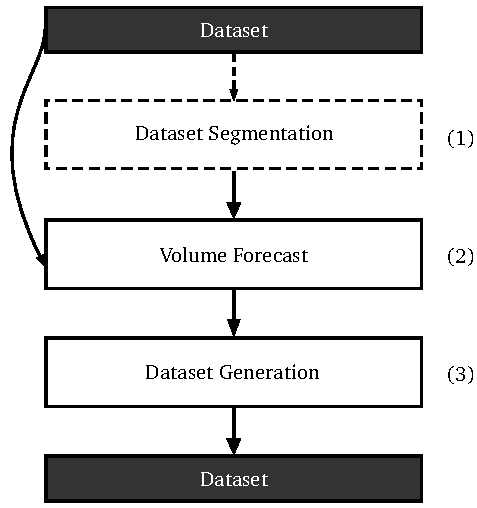
\includegraphics[]{high_level} \caption{ High level overview
of the approach } \label{fig:highlevel_arch} \end{center} \end{figure}

As the figure~\ref{fig:highlevel_arch} makes clear, the goal of the
proposed approach is to use a past dataset containing the log of the web
activity of an online advertising related network to generate a representation of a
possible future web activity on the same network. In such a way, that the
tendencies and the data coherency is preserved.

This approach can be divided three main phases, the first, \emph{segmentation}, is
optional, its main purpose is divide the dataset in smaller and more predictable
datasets in order to improve the results of the second phase, mostly when there
are large quantities of data available.

The second phase is where the \emph{forecast of the volumes} that characterize the traffic on
the network are done, using time series prediction method.

The third an last phase of the process, the more complex one, is where the volumes
generated from the phase two combined with the data provided by the original
dataset are used to \emph{generate a dataset} that represent a possible future of the
web activity on the target network.

\section{Architecture for Web Activity Forecasting and Synthesising}

\subsection{Data Segmentation}

\begin{figure}[h] \begin{center} \leavevmode
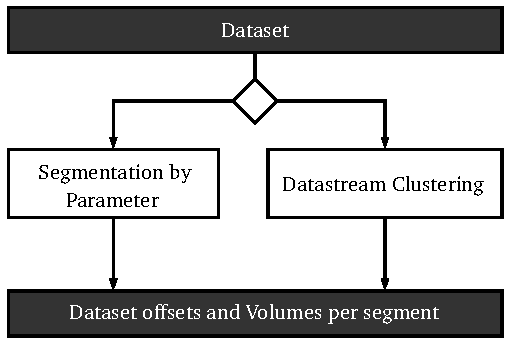
\includegraphics[]{segmentation} \caption{ High level overview
of Data Segmentation} \label{fig:segmentation_arch} \end{center} \end{figure}

The \emph{Data Segmentation} phase was designed in order to achieve better
results in the following phases. 

In order to get better results in the second phase it is need that the time
series obtained from the dataset has certain characteristics that allow it to be
more predictable, a trend and/or a recurring pattern. One way of get the results
is by split the data by some \textbf{parameter} that is known to have effect on the
seasonality of the traffic, for example the website that is being accessed.

As the figure~\ref{fig:segmentation_arch} shows the method described before was
one of the approaches chosen to achieve a more predictable time series. This
method allows to select any parameter available in the dataset and distribute
the impressions clusters. All the members of each cluster share the same value
of the selected parameter. To achieve a good result using this method a great
knowledge about the available impressions is needed.

The other approach that was implemented on this phase is a simplified and
striped down version of a \emph{data stream clustering} algorithm. This
algorithm is distance based, and since the structure of the datasets used on
this thesis are not guaranteed the distance measure used is na\"{i}ve. The
distance between any to impressions can be described as:

\begin{center}
\begin{equation*}
  distance_{x,y}= \sum\limits_{i=0}^n d_i
\end{equation*}
\begin{equation*}
\text{where } d_i = \begin{cases} \text{1 if } x_i = y_x\\
\text{0 otherwise}\end{cases} \text{ and x, y are two impressions from the
dataset}
\end{equation*}
\end{center}

\begin{algorithm}
  \LinesNumbered
  \SetNlSty{texttt}{(}{)}
  \KwData{$lines$, all impressions available on the dataset; $threshold$,
  maximum distance to be considered member of a certain cluster.}
  \KwResult{A list of clusters, each one characterized by the $centroid$ and a list of
  offsets representing the position of each impression on the dataset.}
  \BlankLine

  \Repeat{no more impressions}{
    compare each impression with the existing list of clusters\;
    \eIf{ $dist < threshold$ }{
    add to the selected cluster\;
    }{create a new
    cluster and use the selected impression as the centroid for the new
    cluster\;}
  }
  \BlankLine

  \caption[Data stream clustering]{
    Data stream clustering simplified algorithm to aggregate the impressions by
    the parameters that they have in common.
  }
  \label{alg:pam} \end{algorithm}

This kind of algorithm was selected because of the constrains imposed by the
problem, the most important ones the huge volume of data than this approach
might need to process, the number and type of attributes that compose an
impression can be different from dataset to dataset. The huge volume of data
makes impossible the usage for example of a dissimilarity matrix due to memory
constrains, the uncertainty of the parameters that are available also limit the
quality of the distance measure that assumes that every parameter has the same
weight as the others.

This family of clustering algorithms has some known limitations, for example, the
order in which the dataset is read directly influences the outcome of the
algorithm. Also since the centroids are never updated, as they are represented
by the attributes of the impression that originated that particular centroid,
when a new impression has a distance lower than the threshold when compared with
a certain centroid it is not assured that the respective cluster is the more
similar to the new impression, to address that possible issue the possibility of
search over all available centroids and select the one with a smaller distance
is also available.

\subsection{Volume Forecasting}\label{subsec:volume_forecast}

\begin{figure}[h] \begin{center} \leavevmode
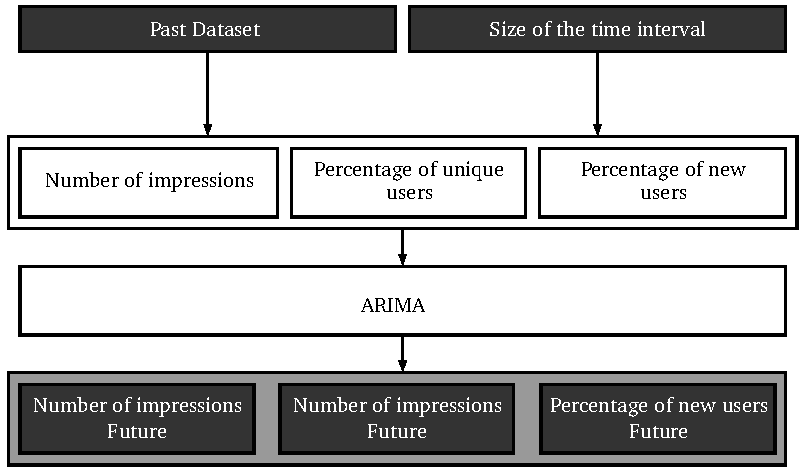
\includegraphics[]{forecast_volumes_arch} \caption{ High level overview
of Data Segmentation} \label{fig:forecast_volumes_arch} \end{center} \end{figure}

One way of describe the impressions is by representing how many happen during a
certain amount of time. So the impressions in the past can be described as time
series, of volume of impressions in time spaced at uniform time intervals. 

So to predict how many impressions will happen in the future time series
analyses techniques can be used. 

Although, the volume of impressions doesn't allow to fully characterize the future so
 it is needed use more time series of different variables that can provide more
 information about each epoch.

The approach here described involves the usage of three time series, one for the
number of impressions, other for the percentage unique users and a last one for
the percentage of unique users that had never appeared in the past.

\paragraph{Number of impressions}
is how many entries are on the dataset during each time interval.

\paragraph{Percentage of unique users}
is described by $\frac{\text{Number of users}}{\text{Number of impressions}}
* 100$, and represents how the number of users are related with the number of
impressions.

\paragraph{Percentage of new users}
represents per unit of time how many users that had never appeared before are
represented. It is described by $\frac{\text{Number of new users}}{\text{Number
of unique users}}*100$.
\\

So each unit of time can be represented by this three values, now to
characterize the future it is needed to forecast each one of this three values
on future time units. To complete this task the \emph{ARIMA} approach was used.


******WHY DID I USED ARIMA

\subsection{Dataset Generator}

\begin{figure}[h] \begin{center} \leavevmode
\includegraphics[]{high_level_file_gen} \caption{ High level overview
of the Dataset Generator } \label{fig:highlevel_arch_file_gen} \end{center} \end{figure}

The last phase of the proposed approach generates a new dataset based on the
original dataset and the values of the three time series generated on the
previous phase.

As shown on figure~\ref{fig:highlevel_arch_file_gen}, this phase was divided in
three sub-phases the pre-process (\ref{subsubsec:pre_process}), calculate
statistics (\ref{subsubsec:stats}) and fill future data
(\ref{subsubsec:fill_data}).

The pre-process sub-phase (\ref{subsubsec:pre_process}), breaks the old dataset in
the interval size that was chosen on the volume prediction phase
(\ref{subsec:volume_forecast}) and organizes the impressions per interval and
users.

The calculate statistics sub-phase (\ref{subsubsec:stats}), uses the processed data
from the past dataset and the volumes from the volume prediction phase
(\ref{subsec:volume_forecast}), verifies if the values make sense in the real
world, for example the number of impressions is higher than the number of users
(it is impossible for this type of dataset to have users with zero impressions,
since the dataset represents impressions), and break the impressions in smaller
intervals and use weekly historical data to predict the distribution of the
interval volumes on the smaller intervals.

The last sub-phase, fill future data (\ref{subsubsec:fill_data}), is the most
crucial phase of this process. It uses the volumes from the last sub-phase, and
then selects past impressions using the restrictions imposed by the calculated volumes. This
phase is also responsible for the generation of new users.

\subsubsection{Pre-process (i)}\label{subsubsec:pre_process}

\begin{figure}[h] \begin{center} \leavevmode
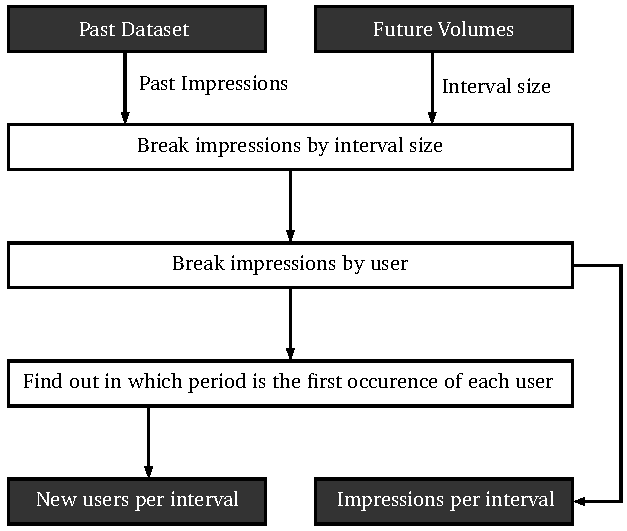
\includegraphics[]{pre_processing_i} \caption{ High level overview
of the Dataset Pre-processing} \label{fig:pre_processing_i} \end{center} \end{figure}

This phase (figure~\ref{fig:pre_processing_i}) can be considered the simpler phase of the whole approach, its main
goal is to provide impressions organized by a defined time interval, and to
place the first occurrence of each user in the correct interval, so the next
phases have the data correctly organized.
\\

This is simply done by reading each line of the dataset and comparing with the
start date of the dataset placing it on the correct interval, also identify
which user is responsible for that impression and, if it is its first occurrence
, place it as a new user for the interval where the impression belong.

\subsubsection{Calculate Statistics (ii)}\label{subsubsec:stats}

\begin{figure}[h] \begin{center} \leavevmode
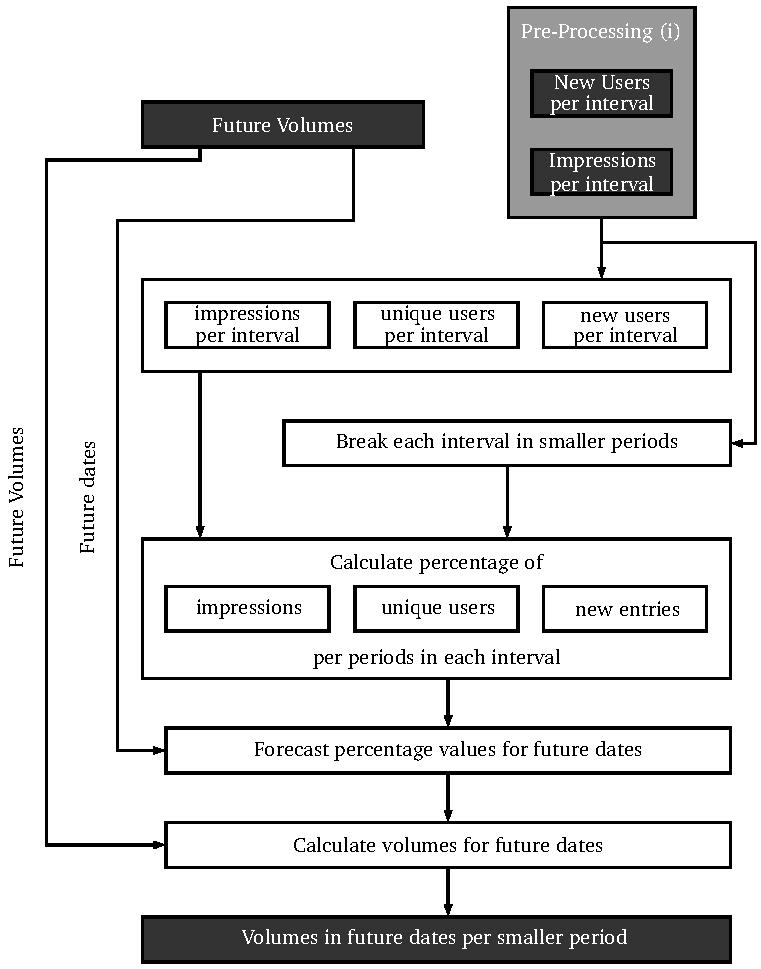
\includegraphics[]{calculate_stats} \caption{ High level overview
of statistics calculation} \label{fig:calculate_stats_ii} \end{center} \end{figure}

The main purpose of the sub-phase represented in the figure~\ref{fig:calculate_stats_ii} is
to distribute the volumes predict for a certain interval in smaller periods
based on historical distribution of the volumes for the same period.

In order to obtain better resolution of how the data is distributed on the
interval, this intervals are broke done in periods of one hour each. Now to
understand how the volumes of the interval are distributed through the periods,
the data from the same interval up to two weeks before the interval which is
being processed is used. For each one hour period of historical interval the
percentage of the total volume is calculated. Then to calculate the distribution
for the current interval the values are the mean of the values of the same interval from the week before
and the week before that, if there is only one week available, then the value of
the current period is the same as the week before, if there are no previous
weeks available then the distribution of the interval volumes is done by
dividing uniformly by each one hour period. After this percentages are
calculated, they are multiplied by the total volumes to obtain the absolute
values for each interval.
\\
For each hour period the following values are calculated:
\begin{itemize}
  \item \textbf{Number of impressions}, this value represents how many requests
    where done during that space in time;
  \item \textbf{Number of users}, number of different users present during that
    space in time;
  \item \textbf{Number of first occurence users}, number of different users that
    occur for the first time in the interval during that specific hour period;
  \item \textbf{Number of new users}, number of different users that are
    completely new to the dataset and occur for the first time in that specific
    hour period.
\end{itemize}

This variables have to respect some constrains in order to be valid. The number
of impressions must be equal or greater than the number of users for a specific
period, the number of users must be less or equal to the sum of number of first
occurrence users, number of new users and number of users that appear on the one
hour periods prior to this period that belong to the same interval. The number
of first occurrence users plus the number of new users must be equal or less
than the number of users for the time period.

So to guarantee integrity of the result that those conditions have to be
fulfilled. So after, the results for the every hour period of a certain interval
of time are calculated, a constrain check must be done and the results must be
adjusted. And to do so the approach implemented on
algorithm~\ref{alg:adjust_values} can be used to fulfil this task.

\begin{algorithm}
  \LinesNumbered
  \SetNlSty{texttt}{(}{)}
  \KwData{$periods$, a list of one tuple for each period; $volumes$,
  a tuple containing the expected values for the interval}
  \KwResult{A list of one tuple for each period, containing the adjusted values
  to meet the imposed constrains}
  \BlankLine

  \While{the sum tuples for all periods != $volumes$}{
    $diff$ = volume - $sum(periods)$\;
    \For{each element of $periods$}{
      To each constrain not respected, change the value acording to the rule and
      then add the difference to the respective $diff$\;
      \If{any constrain not violated and the respective value of $diff$ is not
      0}{ 
        change the respective value while still respect the imposed constrain\;
      }
    }
  }
  \BlankLine

  \caption[Contrain adjustement for statistics]{
    Values adjustment to meet the imposed constrains algorithm
  }
  \label{alg:adjust_values} \end{algorithm}

At the end of this phase we have calculated all the four
values for every future interval for which we want to predict the impressions.


\subsubsection{Fill Future Data (iii)}\label{subsubsec:fill_data}

\begin{figure}[h] \begin{center} \leavevmode
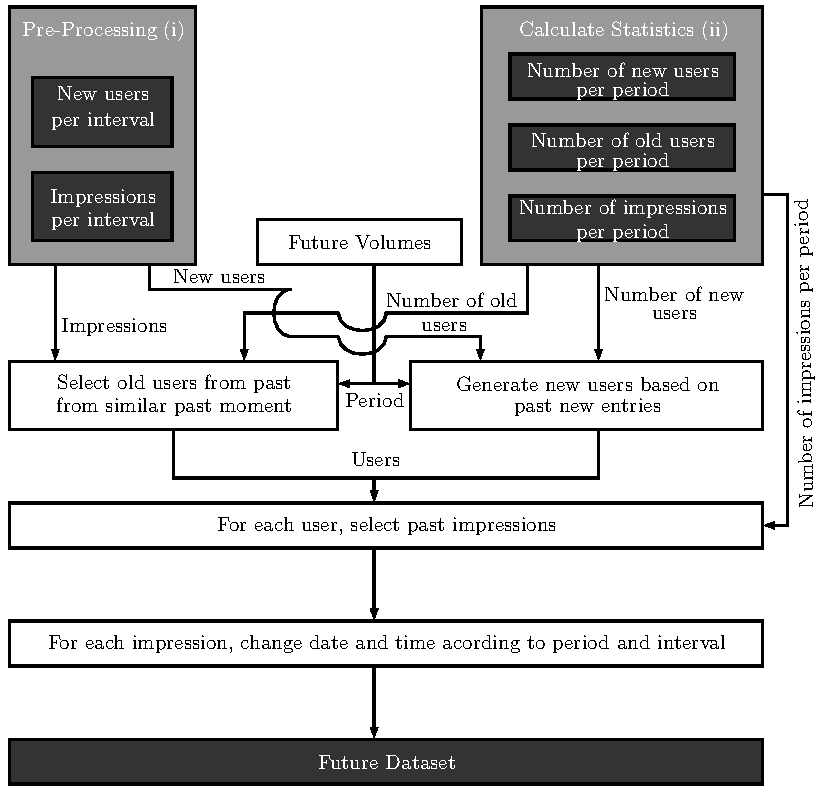
\includegraphics[]{fill_future} \caption{ High level overview
of fill future data} \label{fig:fill_future_iii} \end{center} \end{figure}

placeholder


\section{Component Testing}

\subsection{Data Segmentation}

\subsection{Volume Forecasting}

\subsection{Dataset Generator}


\section{Results and Conclusions}

